\begin{frame}\frametitle{Decadal changes in global ocean chlorophyll} 
\begin{description}
    \item[Authors] Watson W. Gregg, Margarita E. Conkright
    \item[Objectives] The authors aim at finding decadal trends in global ocean chlorophyll between data obtained by CZCS (1979-1986) and those by SeaWiFS (1992– 2000).
    \item[Methods]
        \begin{itemize}
            \item Chlorophyll data from CZCS and SeaWiFS are combined for reanalysis at 1° spatial resolution. 
            \item To increase compatibility and to reduce residual errors, both archives are blended with in situ data. 
        \end{itemize}
\end{description}

  \note[item]{Include notes and talking points here.}
  \note[item]{There can be more than one note.}
\end{frame}

\begin{frame}\frametitle{Decadal changes in global ocean chlorophyll} 
\begin{description}
    \item[Findings] 
        \begin{itemize}
            \item There is large similarity in the global spatial distributions and seasonal variability between the two chlorophyll archives.  
            \item On average, the global ocean chlorophyll has decreased from the CZCS archive to the SeaWiFS by 6\%, and changes are mainly observed in summer and autumn.  
            \item Reductions in North Pacific and North Atlantics in summer are mainly caused by reduced wind stresses and warmer sea surface temperature (SST).  
            \item Regional meteorological events, such as PDP and ENSO have contributed to the changes in global ocean chlorophyll. 
        \end{itemize}
\end{description}
  \note[item]{Include a note if needed.}
\end{frame}

\begin{frame}\frametitle{Decadal changes in global ocean chlorophyll} 
    \hfill
    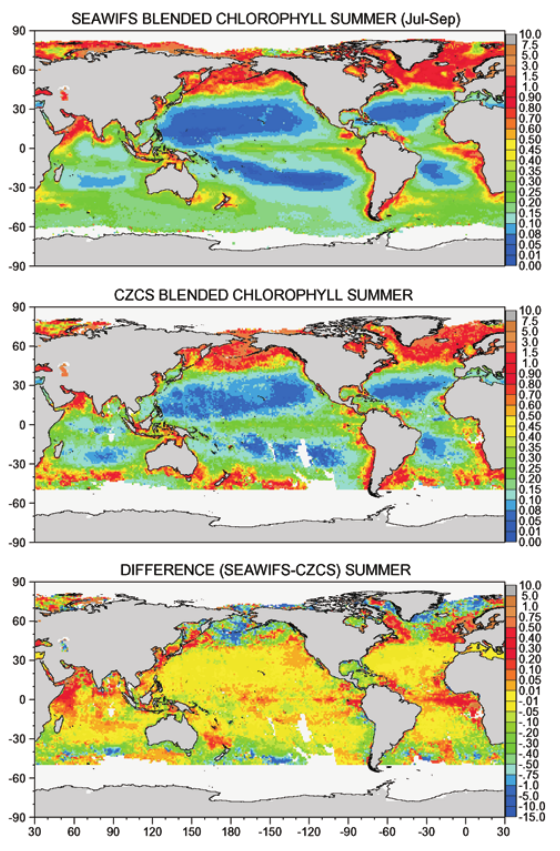
\includegraphics[width=\textwidth,height=0.8\textheight,keepaspectratio]{gregg1}
    \hfill
    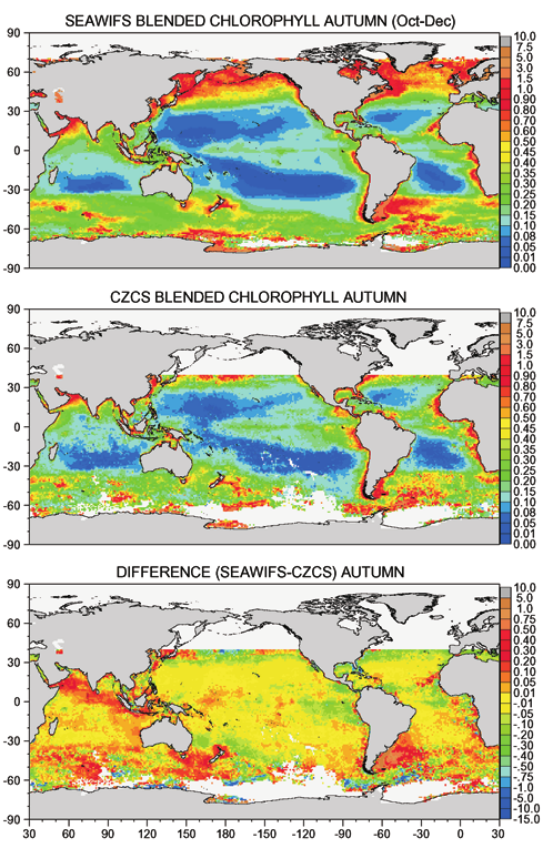
\includegraphics[width=\textwidth,height=0.8\textheight,keepaspectratio]{gregg2}
    \hfill
  \note[item]{Pretty pictures}
\end{frame}
